\documentclass{../../oss-classkick-exam}

\usetikzlibrary{decorations.pathmorphing,patterns}

\begin{document}
\genheader

\gentitle{10}{HARMONIC MOTION}

\genmultidirections

\gengravity

\raggedcolumns
\begin{multicols*}{2}
  \begin{questions}
    \question A mass oscillates hozirontally on the end of a spring that obeys
    Hooke's law. Which of the following statements is true?
    \begin{choices}
      \choice The amplitude of oscillation is equal to the potential energy of
      the spring.
      \choice The kinetic energy of the oscillating mass is constant.
      \choice Maximum potential energy occurs when the mass reaches the
      equilibrium position.
      \choice The potential energy of the spring at the amplitude is equal to
      the kinetic energy at the equilibrium position.
      \choice The kinetic energy of the spring at the amplitude is equal to the
      potential energy.
    \end{choices}
    \vspace{.7in}
    
    \question A superball is dropped from a height of \SI{5.}{\metre} above a
    floor. The ball bounces off the floor in a perfectly elastic collision so
    that it rises to the same height with each bounce. The motion of the ball
    can be described as
    \begin{choices}
      \choice harmonic motion with a period of $2$ \si\second
      \choice harmonic motion with a period of $1$ \si\second
      \choice harmonic motion with a period of $1/2$ \si\second
      \choice motion with a constant velocity
      \choice motion with a constant momentum
    \end{choices}
    \vspace{.7in}
    
    \question An object oscillates in simple harmonic motion along the $x$-axis
    according to the equation $x=6\cos(4t)$. The period of oscillation of the
    object is
    \begin{choices}
      \choice $1/4$ s
      \choice 4 s
      \choice $\pi/4$ s
      \choice $\pi/2$ s
      \choice $4\pi$ s
    \end{choices}
    
%    \question A mass $m$ oscillates on the end of a string of length $L$. The
%    frequency of the pendulum is $f$. How would you increase the frequency of
%    the pendulum to $2f$?
%    \begin{center}
%      \begin{tikzpicture}[scale=1.1]
%        \fill [pattern=north east lines] (-2,4) rectangle (2,4.2);
%        \draw[ultra thick] (-2,4)--(2,4);
%        \draw[thick,
%          decoration={aspect=.3,segment length=2mm, amplitude=2.5mm, coil},
%          decorate] (-1,4)--(-1,3);
%        \draw[thick,
%          decoration={aspect=.3,segment length=2mm, amplitude=2.5mm, coil},
%          decorate] (1,4)--(1,3);
%        \draw[fill=gray!70](-1.5,3) rectangle(1.5,2);
%      \end{tikzpicture}
%    \end{center}
%    \begin{choices}
%      \choice Increase the length of the pendulum to $4L$
%      \choice Decrease the length of the pendulum to $L/4$
%      \choice Increase the length of the pendulum to $2L$
%      \choice Decrease the length of the pendulum to $L/2$
%      \choice Decrease the mass of the pendulum to $m/2$
%    \end{choices}
%    \vspace{.7in}
    
    \question A mass hangs from two parallel springs, each with the same spring
    constant $k$. Compared to the period $T$ of the same mass oscillating on
    one of the springs, the period of oscillation of the mass with both
    springs connected to it is
    \begin{choices}
      \choice $T/2$
      \choice $T/\sqrt2$
      \choice $T$ (unchanged)
      \choice $\sqrt2T$
      \choice $2T$
    \end{choices}
    \columnbreak
    
    \question Which of the following is generally true for an object in simple
    harmonic motion on a spring of constant $k$?
    \begin{choices}
      \choice The greater the spring constant $k$, the greater the amplitude of
      the motion.
      \choice The greater the spring constant $k$, the greater the period of
      the motion.
      \choice The greater the spring constant $k$, the greater the frequency of
      the motion.
      \choice The lower the spring constant $k$, the greater the frequency of
      the motion.
      \choice The lower the spring constant $k$, the greater the kinetic energy
      of the motion.
    \end{choices}
    \vspace{.7in}

    \uplevel{  
      \textbf{Questions \ref{first}--\ref{last}}

      A harmonic oscillator follows the equation $\dfrac{d^2x}{dt^2}=-4x$. The
      spring constant $k$ is \SI4{\newton\per\metre}.
    }

    \question The angular frequency $\omega$ of the harmonic motion is
    \begin{choices}
      \choice zero
      \choice\SI2{rad\per\second}
      \choice\SI4{rad\per\second}
      \choice\SI8{rad\per\second}
      \choice\SI{16}{rad\per\second}
    \end{choices}
    \label{first}

    \question The mass $m$ oscillating on the spring is
    \begin{choices}
      \choice\SI{1}{\kilo\gram}
      \choice\SI{2}{\kilo\gram}
      \choice\SI{4}{\kilo\gram}
      \choice\SI{8}{\kilo\gram}
      \choice\SI{16}{\kilo\gram}
    \end{choices}
    
    \question The period $T$ of oscillation is
    \begin{choices}
      \choice zero
      \choice $\pi/4$\si\second
      \choice $\pi/2$\si\second
      \choice $\pi$  \si\second
      \choice $2\pi$ \si\second
    \end{choices}
    \label{last}
    
    \question A pendulum of length $L$ has a period of \SI2{\second} on Earth.
    A planetary explorer takes the same pendulum of length $L$ to another
    planet where its period is \SI1\second. The gravitational acceleration on
    the surface of this planet is most nearly
%    \begin{center}
%      \begin{tikzpicture}
%        \fill [pattern=north east lines] (-5,0)--(0,0)--(0,2)--(.2,2)--
%        (.2,-.2)--(-5,-.2)--cycle;
%        \draw[ultra thick] (-5,0)--(0,0)--(0,2);
%        \draw[decoration={aspect=.3,segment length=2mm, amplitude=2.5mm, coil},
%          decorate] (0,.5)--(-1,.5);
%        \draw[fill=gray!70](-2,0) rectangle(-1,1) node[above]{\SI{1}{\kg}};
%        \draw[fill=gray!70](-4.5,0) rectangle(-3.5,1) node[above]{\SI{1}{\kg}};
%        \draw[ultra thick,->](-4,.5)--(-2.8,.5) node[pos=1,right]{$v$};
%        \draw[very thick,dashed](-.5,-.5)--(-.5,1.5);
%      \end{tikzpicture}
%    \end{center}
    \begin{choices}
      \choice$8g$
      \choice$4g$
      \choice$2g$
      \choice$g/2$
      \choice$g/4$
    \end{choices}
  \end{questions}
\end{multicols*}
\newpage

\genfreetitle{10}{HARMONIC MOTION}{4}

\genfreedirections

\begin{questions}
%\item A mass $m$ oscillates on an ideal spring of spring constant $k$ on a
%  frictionless horizontal surface. The mass is pulled aside to a distance $A$
%  from its equilibrium position, and released.
%  \begin{center}
%    \begin{tikzpicture}
%      \fill [pattern=north east lines] (5,0)--(0,0)--(0,2)--(-0.2,2)
%      --(-0.2,-0.2)--(5,-0.2)--cycle;
%      \draw[ultra thick] (5,0)--(0,0)--(0,2)--(-0.5,2);
%      \draw[decoration={aspect=0.3,segment length=2mm, amplitude=2.5mm, coil},
%        decorate] (0,0.5)--(1.5,0.5);
%      \draw[fill=gray!70](1.5,0) rectangle(2.5,1);
%      \draw[thick](2.5,0)--(2.5,-0.3) node[pos=1,below]{O};
%      \draw[thick](4,0)--(4,-0.3) node[pos=1,below]{A};
%    \end{tikzpicture}
%  \end{center} 
%  \begin{enumerate}[noitemsep]  
%  \item In terms of the given quantities, at what distance from the equilibrium
%    position is the potential energy of the mass equal to its kinetic energy?
%  \item In terms of the given quantities, what is the acceleration of the mass
%    when it is at the amplitude $A$?
%  \end{enumerate}
%%  \vspace{3in}
%  \newpage


% THIS QUESTION SHOULD MOVE TO AP/IBHL PHYSICS 
%  \question Show that for the situations in the figures below, the object of
%  mass $m$ oscillates with a frequency of
%  $f=\dfrac1{2\pi}\sqrt{\dfrac{k_\text{eff}}m}$ where $k_\text{eff}$
%  is given by (a) $k_\text{eff}=k_1+k_2$ and (b)
%  $\displaystyle\frac1{k_\text{eff}}=\frac1{k_1}+\frac1{k_2}$. Hint:
%  find the net force on the mass and write $F=-k_\text{eff}x$. Note that in
%  (b), the springs stretch by different amounts, the sum of which is $x$.
%  
%  (a)\hspace{5pt}
%  \begin{tikzpicture}[scale=.5]
%    \fill[gray!50](0,0) rectangle(12,-.75);
%    \fill[gray!50](-.75,-.75) rectangle(0,3);
%    \fill[gray!50](12,-.75) rectangle(12.75,3);
%    \fill[yellow!80!gray](5.25,0) rectangle(6.75,1.5) node[midway,black]{$m$};
%    \draw[decoration={aspect=0.3,segment length=2mm, amplitude=1.25mm, coil},
%      decorate] (0,.75)--(5.25,.75) node[midway,above]{$k_1$};
%    \draw[decoration={aspect=0.3,segment length=2mm, amplitude=1.25mm, coil},
%      decorate] (6.75,.75)--(12,.75) node[midway,above]{$k_2$};
%    \draw[very thick](0,3)--(0,0)--(12,0)--(12,3);
%  \end{tikzpicture}
%
%  (b)\hspace{5pt}
%  \begin{tikzpicture}[scale=.5]
%    \fill[gray!50](0,0) rectangle(12.75,-.75);
%    \fill[gray!50](-.75,-.75) rectangle(0,3);
%    \fill[yellow!80!gray](10.5,0) rectangle(12,1.5) node[midway,black]{$m$};
%    \draw[decoration={aspect=0.3,segment length=2mm, amplitude=1.25mm, coil},
%      decorate] (0,.75)--(6,.75) node[midway,above]{$k_1$};
%    \draw[decoration={aspect=0.3,segment length=2mm, amplitude=1.25mm, coil},
%      decorate] (6,.75)--(10.5,.75) node[midway,above]{$k_2$};
%    \fill[black](6,.75) circle(.15);
%    \draw[very thick](0,3)--(0,0)--(12.75,0);
%  \end{tikzpicture}
%  \newpage
  
  \question A simple pendulum of length $L$ is released from rest from an angle
  of $\theta_0$.
  \begin{parts}
    \part Assuming the motion of the pendulum to be simple harmonic motion, find
    its speed as it passes through $\theta=0$.
    \part Using the conservation of energy, find this speed exactly.
    \part Show that your results for (a) and (b) are the same when $\theta_0$ is
    small.
    \part Find the difference in your results for $\theta_0=\SI{.20}{rad}$ and
    $L=\SI1\metre$.
  \end{parts}
  \newpage
    
  \uplevel{
    \cpic{.35}{torsional}
  }  
  \question The torsion pendulum shown above consists of a disk of rotational
  inertia $I$ suspended by a flexible rod attached to a rigid support. When the
  disk is twisted through a small angle $\theta$, the twisted rod exerts a
  restoring torque $\tau$ that is proportional to the angular displacement:
  $\tau=-\beta\theta$, where $\beta$ is a constant. The motion of a torsion
  pendulum is analogous to the motion of a mass oscillating on a spring.
  \begin{parts}
    \part In terms of the quantities given above, write but do NOT solve the
    differential equation that could be used to determine the angular
    displacement $\theta$ of the torsion pendulum as a function of time $t$.
    
    \part Using the analogy to a mass oscillating on a spring, determine the
    period of the torsion pendulum in terms of the given quantities and
    fundamental constants, as appropriate.

    \uplevel{
      To determine the torsion constant $\beta$ of the rod, disks of different,
      known values of rotational inertia are attached to the rod, and the data
      below are obtained from the resulting oscillations.
      \begin{center}
        \begin{tabular}{|c|c|c|c|}
          \hline
          Rotational Inertia $I$ of Disk (\si{\kilo\gram\metre\squared}) &
          Average Time for Ten Oscillations (s) &
          Period $T$ (s) & $T^2$ (\si{\second\squared}) \\\hline
          0.025 & 22.4 & 2.24 & 5.0  \\\hline
          0.036 & 26.8 & 2.68 & 7.2  \\\hline
          0.049 & 29.5 & 2.95 & 8.7  \\\hline
          0.064 & 33.3 & 3.33 & 11.1 \\\hline
          0.081 & 35.9 & 3.59 & 12.9 \\\hline
        \end{tabular}
      \end{center}
    }
  
    \part On the graph below, plot the data points. Draw a straight line that
    best represents the data.
    \cpic{.9}{graph-paper}
 
    \part Determine the equation for your line.
 
    \part Calculate the torsion constant $\beta$ of the rod from your line.
 
    \part What is the physical significance of the intercept of your line with
    the vertical axis?
  \end{parts}
  \newpage

  % TAKEN FROM 2012 AP PHYSICS C MECHANICS EXAM FREE-RESPONSE QUESTION 1
  \uplevel{
    \cpic{.5}{spring-mass}
  }
  \question \underline{Experiment 1.} A block of mass 0.30 kg is placed on a
  frictionless table and is attached to one end of a horizontal spring of
  spring constant $k$, as shown above. The other end of the spring is attached
  to a fixed wall. The block is set into oscillatory motion by stretching the
  spring and releasing the block from rest at time $t=0$. A motion detector is
  used to record the position of the block as it oscillates. The resulting
  graph of velocity $\varv$ versus time $t$ is shown below. The positive
  direction for all quantities is to the right.
  \cpic{.5}{oscillation1}
  \begin{parts}
    \part Determine the equation for $\varv(t)$, including numerical values for
    all constants.
 
    \part Given that the equilibrium position is at $x=0$, determine the
    equation for $x(t)$, including numerical values for all constants.

    \part Calculate the value of $k$.
    \newpage
    
    \uplevel{
      \underline{Experiment 2.} The block and spring arrangement is now
      placed on a rough surface, as shown below. The block is displaced so that
      the spring is \underline{compressed} a distance $d$ and released from
      rest.
      \begin{center}
        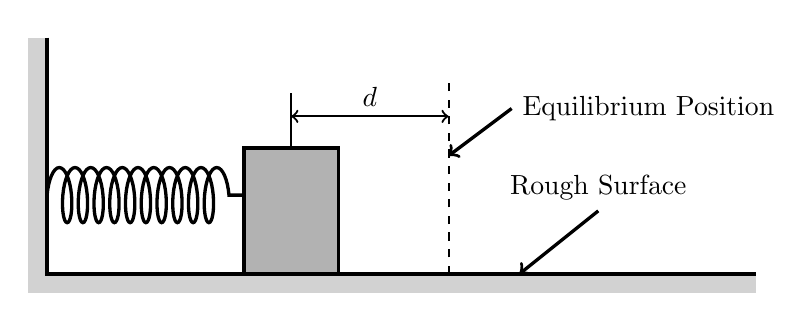
\begin{tikzpicture}
          \draw[lightgray!70,line width=7.2](-.12,3)--(-.12,-.12)--(9,-.12);
          \draw[very thick](0,3)--(0,0)--(9,0);
          \draw[dashed,thick](5.1,0)--(5.1,2.5);
          \draw[thick](3.1,1.6)--(3.1,2.3);
          \draw[very thick,fill=gray!60](2.5,0) rectangle (3.7,1.6);
          \draw[thick,<->](3.1,2)--(5.1,2) node[midway,above]{$d$};
          \draw[very thick,<-](6,0)--(7,.8) node[above]{Rough Surface};
          \draw[very thick,<-](5.1,1.5)--(5.9,2.1)
          node[right]{Equilibrium Position};
          \draw[very thick,
        decoration={aspect=.3,segment length=2mm, amplitude=3.5mm, coil},
        decorate] (0,1)--(2.5,1);
        \end{tikzpicture}
      \end{center}
    }
    \part On the dots below that represent the block, draw and label the forces
    (not components) that act on the block when the spring is
    \underline{compressed} a distance $x=d/2$ and the block is moving in the
    direction indicated below each dot.
    
    \begin{minipage}{.45\textwidth}
      \vspace{.8in}
      \begin{center}
        \tikz{\fill circle(.15);}
        
        \vspace{.5in}
        Toward\\
        the equilibrium position
      \end{center}
    \end{minipage}
    \begin{minipage}{.45\textwidth}
      \vspace{.8in}
      \begin{center}
        \tikz{\fill circle(.15);}
        
        \vspace{.5in}
        Away from\\
        the equilibrium position
      \end{center}
    \end{minipage}
    
    \part Draw a sketch of $\varv$ versus $t$ in this case. Assume that
    there is a negligible change in the period and that the positive direction
    is still to the right.
    \uplevel{
      \centering
      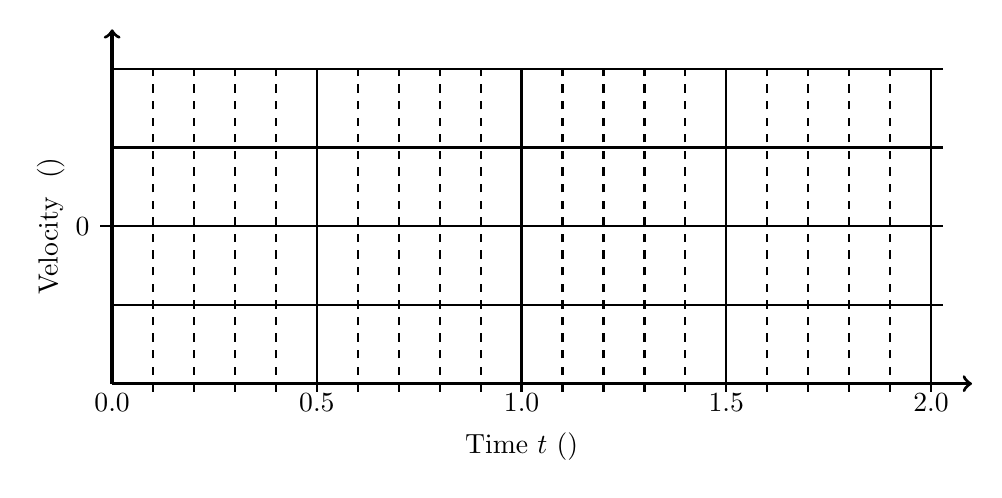
\begin{tikzpicture}[xscale=5.2]
        \begin{scope}[very thick,->]
          \draw(0,-2)--(2.1,-2);
          \draw(0,-2)--(0,2.5);
        \end{scope}
        \foreach \x in {0.1,0.2,...,2.0}\draw[dashed,thick](\x,-2.1)--(\x,2);
        \foreach \x in {0.0,0.5,1.0,1.5,2.0}
        \draw[thick](\x,-2)--(\x,2) node[pos=0,below]{$\x$};
        \foreach \y in {-1,...,2}\draw[thick](0,\y)--(2.03,\y);
        \draw[thick](0,0)--(-0.03,0) node[left]{$0$};
        \node at (1,-2.8){Time $t$ (\si\second)};
        \node[rotate=90] at (-.15,0){Velocity $\varv$ (\si{\metre\per\second})};
      \end{tikzpicture}
    }
  \end{parts}
  \newpage
  
  % TAKEN FROM 2003 AP PHYSICS C MECHANICS EXAM FREE-RESPONSE QUESTION 2
  \uplevel{
    \cpic{.3}{hung-spring}
  }
  \question An ideal spring is hung from the ceiling and a pan of mass $M$ is
  suspended from the end of the spring, stretching it a distance $D$ as shown
  above. A piece of clay, also of mass $M$, is then dropped from a height $H$
  onto the pan and sticks to it. Express all algebraic answers in terms of the
  given quantities and fundamental constants.
  \begin{parts}
    \part Determine the speed of the clay at the instant it hits the pan.
    \part Determine the speed of the pan just after the clay strikes it.
    \part Determine the period of the simple harmonic motion that ensues.
    \part Determine the distance the spring is stretched (from its initial
    unstretched length) at the moment the speed of the pan is a maximum.
    Justify your answer.

    \part The clay is now removed from the pan and the pan is returned to
    equilibrium at the end of the spring. A rubber ball, also of mass $M$, is
    dropped from the same height H onto the pan, and after the collision is
    caught in midair before hitting anything else.
    
    Indicate below whether the period of the resulting simple harmonic motion
    of the pan is greater than, less than, or the same as it was in part (c).
    Justify your answer.
    
    \vspace{.1in}
    \underline{\hspace{.3in}} Greater than\hspace{.4in}
    \underline{\hspace{.3in}} Less than\hspace{.4in}
    \underline{\hspace{.3in}} The same as
  \end{parts}
\end{questions}
\end{document}
